% Template for Elsevier CRC journal article
% version 1.2 dated 09 May 2011

% This file (c) 2009-2011 Elsevier Ltd.  Modifications may be freely made,
% provided the edited file is saved under a different name

% This file contains modifications for Procedia Computer Science

% Changes since version 1.1
% - added "procedia" option compliant with ecrc.sty version 1.2a
%   (makes the layout approximately the same as the Word CRC template)
% - added example for generating cThe error distribution analysis reveals a slight positive bias (mean error 0.109), suggesting minor tendency to overestimate returns. Notably, 76\% of prediction errors fall within the ±0.3 range, indicating consistent performance across most stock instances. These results demonstrate the model's utility for real-world applications such as portfolio allocation, trend forecasting, and quantitative screening, maintaining high alignment with actual movements despite market noise.right line in abstract

%-----------------------------------------------------------------------------------

%% This template uses the elsarticle.cls document class and the extension package ecrc.sty
%% For full documentation on usage of elsarticle.cls, consult the documentation "elsdoc.pdf"
%% Further resources available at http://www.elsevier.com/latex

%-----------------------------------------------------------------------------------

%%%%%%%%%%%%%%%%%%%%%%%%%%%%%%%%%%%%%%%%%%%%%%%%%%%%%%%%%%%%%%
%%%%%%%%%%%%%%%%%%%%%%%%%%%%%%%%%%%%%%%%%%%%%%%%%%%%%%%%%%%%%%
%%                                                          %%
%% Important note on usage                                  %%
%% -----------------------                                  %%
%% This file should normally be compiled with PDFLaTeX      %%
%% Using standard LaTeX should work but may produce clashes %%
%%                                                          %%
%%%%%%%%%%%%%%%%%%%%%%%%%%%%%%%%%%%%%%%%%%%%%%%%%%%%%%%%%%%%%%
%%%%%%%%%%%%%%%%%%%%%%%%%%%%%%%%%%%%%%%%%%%%%%%%%%%%%%%%%%%%%%

%% The '3p' and 'times' class options of elsarticle are used for Elsevier CRC
%% The 'procedia' option causes ecrc to approximate to the Word template
\documentclass[3p,times,procedia]{elsarticle}
\flushbottom

% Space optimization commands
\setlength{\parskip}{3pt}
\setlength{\baselineskip}{11pt}
\addtolength{\textfloatsep}{-4pt}
\addtolength{\floatsep}{-3pt}
\addtolength{\intextsep}{-3pt}

%% The `ecrc' package must be called to make the CRC functionality available
\usepackage{ecrc}
\usepackage[utf8]{inputenc}
\usepackage{amssymb}
\usepackage{multicol}
\usepackage[table,xcdraw]{xcolor}
\usepackage{graphicx}
\usepackage{cellspace}
\usepackage{longtable}
\usepackage{tipa}
\usepackage{amsmath}
\usepackage{amsfonts}
\usepackage{pdfpages}
\usepackage{footnote}
\usepackage{amsthm}
\usepackage{rotating}
\usepackage{multirow}
\usepackage[justification=justified, format=plain]{caption}
\usepackage{relsize}
\usepackage[bookmarks=false]{hyperref}
    \hypersetup{colorlinks,
      linkcolor=blue,
      citecolor=blue,
      urlcolor=blue}
\usepackage{url}
\urlstyle{same}  % Use same font as text for URLs
\usepackage{pifont}
%\usepackage[ruled,vlined,linesnumbered]{algorithm2e}  %nofillcomment, noend
\usepackage{etoolbox}
\usepackage{lipsum}% just to generate some text
\usepackage[english]{babel}
\usepackage[T1]{fontenc}
\usepackage{wrapfig, blindtext}
\usepackage{stackengine}
\usepackage{tabulary}
\usepackage{url}
% \usepackage[noadjust]{cite}  % Conflicts with natbib already loaded by elsarticle
\usepackage{amstext}
\usepackage{array,times}
\usepackage{booktabs,chemformula}
\usepackage[cal=boondox]{mathalfa}
\usepackage[mathscr]{eucal}
\usepackage[newcommands]{ragged2e}
\usepackage{bm}
% \usepackage{cite}  % Conflicts with natbib already loaded by elsarticle
\usepackage{amsmath,amssymb,amsfonts,bm}
\usepackage{float}      % Required for [H] option
\usepackage{placeins}   % Required for \FloatBarrier
% \usepackage{caption}    % Already loaded above with options
\usepackage{booktabs}
\usepackage{tabularx} % For the tabularx environment
\usepackage{algorithm}
\usepackage{algpseudocode}
\usepackage{array}  % Improve table formatting
\usepackage{textcomp}
\usepackage{adjustbox}
\usepackage{verbatim}
\usepackage{listings}
\def\BibTeX{{\rm B\kern-.05em{\sc i\kern-.025em b}\kern-.08em
T\kern-.1667em\lower.7ex\hbox{E}\kern-.125emX}}

%% The ecrc package defines commands needed for running heads and logos.
%% For running heads, you can set the journal name, the volume, the starting page and the authors

%% set the volume if you know. Otherwise `00'
\volume{00}

%% set the starting page if not 1
\firstpage{1}

%% Give the name of the journal
\journalname{Procedia Computer Science}

%% Give the author list to appear in the running head
%% Example \runauth{C.V. Radhakrishnan et al.}
\runauth{Author name}

%% The choice of journal logo is determined by the \jid and \jnltitlelogo commands.
%% A user-supplied logo with the name <\jid>logo.pdf will be inserted if present.
%% e.g. if \jid{yspmi} the system will look for a file yspmilogo.pdf
%% Otherwise the content of \jnltitlelogo will be set between horizontal lines as a default logo

%% Give the abbreviation of the Journal.
\jid{procs}

%% Give a short journal name for the dummy logo (if needed)
%\jnltitlelogo{Computer Science}

%% Hereafter the template follows `elsarticle'.
%% For more details see the existing template files elsarticle-template-harv.tex and elsarticle-template-num.tex.

%% Elsevier CRC generally uses a numbered reference style
%% For this, the conventions of elsarticle-template-num.tex should be followed (included below)
%% If using BibTeX, use the style file elsarticle-num.bst

%% End of ecrc-specific commands
%%%%%%%%%%%%%%%%%%%%%%%%%%%%%%%%%%%%%%%%%%%%%%%%%%%%%%%%%%%%%%%%%%%%%%%%%%

%% The amssymb package provides various useful mathematical symbols
% (already loaded above)
% \usepackage{amssymb}
%% The amsthm package provides extended theorem environments
%% \usepackage{amsthm}

%% The lineno packages adds line numbers. Start line numbering with
%% \begin{linenumbers}, end it with \end{linenumbers}. Or switch it on
%% for the whole article with \linenumbers after \end{frontmatter}.
%% \usepackage{lineno}

%% natbib.sty is loaded by default. However, natbib options can be
%% provided with \biboptions{...} command. Following options are
%% valid:

%%   round  -  round parentheses are used (default)
%%   square -  square brackets are used   [option]
%%   curly  -  curly braces are used      {option}
%%   angle  -  angle brackets are used    <option>
%%   semicolon  -  multiple citations separated by semi-colon
%%   colon  - same as semicolon, an earlier confusion
%%   comma  -  separated by comma
%%   numbers-  selects numerical citations
%%   super  -  numerical citations as superscripts
%%   sort   -  sorts multiple citations according to order in ref. list
%%   sort&compress   -  like sort, but also compresses numerical citations
%%   compress - compresses without sorting
%%
%% \biboptions{authoryear}

\biboptions{numbers}

% if you have landscape tables

%\usepackage{harvard}
% put your own definitions here:x
%   \newcommand{\cZ}{\cal{Z}}
%   \newtheorem{def}{Definition}[section]
%   ...

% add words to TeX's hyphenation exception list
%\hyphenation{author another created financial paper re-commend-ed Post-Script}

% declarations for front matter


\begin{document}
\begin{frontmatter}

%% Title, authors and addresses

%% use the tnoteref command within \title for footnotes;
%% use the tnotetext command for the associated footnote;
%% use the fnref command within \author or \address for footnotes;
%% use the fntext command for the associated footnote;
%% use the corref command within \author for corresponding author footnotes;
%% use the cortext command for the associated footnote;
%% use the ead command for the email address,
%% and the form \ead[url] for the home page:
%%
%% \title{Title\tnoteref{label1}}
%% \tnotetext[label1]{}
%% \author{Name\corref{cor1}\fnref{label2}}
%% \ead{email address}
%% \ead[url]{home page}
%% \fntext[label2]{}
%% \cortext[cor1]{}
%% \address{Address\fnref{label3}}
%% \fntext[label3]{}

\dochead{International Conference on Machine Learning and Data Engineering (ICMLDE 2025)}%%%
%% Use \dochead if there is an article header, e.g. \dochead{Short communication}
%% \dochead can also be used to include a conference title, if directed by the editors
%% e.g. \dochead{17th International Conference on Dynamical Processes in Excited States of Solids}

\title{FinReport: Explainable Stock Earnings Forecasting via News Factor Analyzing Model}

%% use optional labels to link authors explicitly to addresses:
%% \author[label1,label2]{<author name>}
%% \address[label1]{<address>}
%% \address[label2]{<address>}



\author[a]{Mukesh Kumar}
\author[b]{Md Azlan}
\author[c]{Kanishk}
\author[d]{Kingshuk Chatterjee}
\author[e]{Gopesh Satapathy}

\address[a]{School of Computer Engineering, Kalinga Institute of Industrial Technology, Bhubaneswar-751024, India}
\address[b]{School of Computer Engineering, Kalinga Institute of Industrial Technology, Bhubaneswar-751024, India}
\address[c]{School of Computer Engineering, Kalinga Institute of Industrial Technology, Bhubaneswar-751024, India}
\address[d]{School of Computer Engineering, Kalinga Institute of Industrial Technology, Bhubaneswar-751024, India}
\address[e]{School of Computer Engineering, Kalinga Institute of Industrial Technology, Bhubaneswar-751024, India}



\begin{abstract}
%% Text of abstract
Financial market forecasting has become increasingly challenging, as traditional technical analysis does not capture rapid volatility and sentiment-driven price movements. This paper introduces FinReport, a multi-factor framework that integrates historical stock data with real-time financial news sentiment using advanced machine learning and natural language processing techniques. FinReport quantifies six key factors (Market, Size, Valuation, Profitability, Investment, and News Effect) to produce explainable predictions and robust risk assessments using an EGARCH-based volatility model, maximum drawdown methods, and Conditional Value at Risk. Empirical results on 75 Chinese A-share stocks (2018-2021) demonstrate superior performance: mean RMSE 0.2546, MAE 0.2433, $R^2 = 0.5515$ with 15\% RMSE and 12\% MAE reduction versus LSTM baselines. Top performers achieve $R^2 > 0.98$ (7.1\% of stocks), with 20\% Sharpe ratio improvement and prediction-actual correlation $\rho = 0.948$. Cross-validation confirms model stability across temporal folds ($R^2$: 0.523-0.585).
\end{abstract}

\begin{keyword}
Financial forecasting, stock market prediction, multi-factor analysis, technical indicators, financial news sentiment, natural language processing, machine learning, EGARCH, LSTM, risk assessment, explainable AI, FinReport.

%% keywords here, in the form: keyword \sep keyword

%% PACS codes here, in the form: \PACS code \sep code

%% MSC codes here, in the form: \MSC code \sep code
%% or \MSC[2008] code \sep code (2000 is the default)

\end{keyword}
\cortext[cor1]{Mukesh Kumar}
\end{frontmatter}

%\correspondingauthor[*]{Corresponding author. Tel.: +0-000-000-0000 ; fax: +0-000-000-0000.}
\email{mukesh.kumarfcs@kiit.ac.in}

%%
%% Start line numbering here if you want
%%
% \linenumbers

%% main text

% Copyright and publication information
\vspace{8pt}
\noindent\textbf{Mukesh Kumar}\\
E-mail address: mukesh.kumarfcs@kiit.ac.in

\vspace{4pt}
\noindent 1877-0509 \copyright\ 2025 The Authors. Published by Elsevier B.V.\\
This is an open access article under the CC BY-NC-ND license (http://creativecommons.org/licenses/by-nc-nd/4.0/)\\
Peer-review under responsibility of the scientific committee of the International Conference on Machine Learning and Data Engineering.

\vspace{6pt}

\section{Introduction}
\label{main}

Financial markets exhibit unprecedented volatility, with emerging markets like the Shanghai Stock Exchange showing daily volatility of 1.7\% versus 0.8-1.2\% for developed markets. Traditional econometric models such as ARIMA \cite{Box1970} struggle to capture sentiment-driven price movements and complex market interdependencies \cite{FAMA1993}. The efficient market hypothesis faces challenges from documented predictable patterns and behavioral factors.

We propose FinReport, a multi-factor framework integrating historical stock data with financial news via machine learning and NLP techniques \cite{Bao2017}. Unlike traditional quantitative approaches, FinReport leverages structured numerical and unstructured textual data for enhanced prediction accuracy. The framework computes six factors (market, size, valuation, profitability, investment, and news effect) for explainable predictions with EGARCH-based risk assessment \cite{Nelson1991}.

Experimental results on Chinese A-share stocks (2018-2021) \cite{FinReportDataset2025} demonstrate 15\% RMSE reduction, 12\% MAE reduction versus LSTM baselines \cite{Fischer2018}, and 20\% Sharpe ratio improvement. This work bridges traditional econometric methods with explainable AI \cite{TETLOCK2007,Ribeiro2016}, advancing computational finance through interpretable sentiment-quantitative integration.

\textbf{Paper Organization:} Section 2 reviews related literature. Section 3 presents the FinReport system architecture. Section 4 details algorithmic implementations. Section 5 provides experimental results. Section 6 concludes with limitations and future guidance.




\section{Literature Review}

Early forecasting methods like ARIMA \cite{Box1970} underperformed with RMSE exceeding 0.05 during volatile periods. Multi-factor models by Fama and French \cite{FAMA1993} improved performance but ignored qualitative inputs. LSTM networks \cite{Fischer2018} capture long-term dependencies achieving $R^2 \approx 0.45$ on financial datasets. Recent work integrates financial news sentiment using FinBERT \cite{Araci2019} and NLP frameworks \cite{Loughran2011}, showing 12\% prediction improvement.

\textbf{Comparative Performance:} Bao et al. \cite{Bao2017} reported $R^2 = 0.42$ using stacked autoencoders. Nelson's EGARCH \cite{Nelson1991} achieved volatility prediction accuracy of 78\%. Tetlock's sentiment analysis \cite{TETLOCK2007} demonstrated 15\% return predictability. Our FinReport framework achieves superior $R^2 = 0.5515$, representing 31\% improvement over LSTM baselines and 15\% over recent sentiment-enhanced models.

However, traditional approaches lack interpretability \cite{Ribeiro2016}, motivating explainable AI frameworks combining structured numerical with unstructured text analysis. The literature increasingly advocates for explainable models that combine structured numerical data with unstructured text analysis, setting the stage for FinReport's factor-based approach to transparent and robust financial forecasting.

\section{System Model And Proposed Mechanism}

FinReport integrates traditional multi-factor models \cite{FAMA1993,Carhart1997} with real-time news sentiment analysis \cite{TETLOCK2007}, extending established financial theory to capture behavioral market dynamics \cite{Daniel1998}. The system employs a modular design with five interconnected components: (1) Data Integration, (2) News Factor Extraction, (3) Return Forecasting, (4) Risk Assessment, and (5) Dynamic Report Generation \cite{Fischer2018}.

\begin{figure}[!ht]
    \centering
    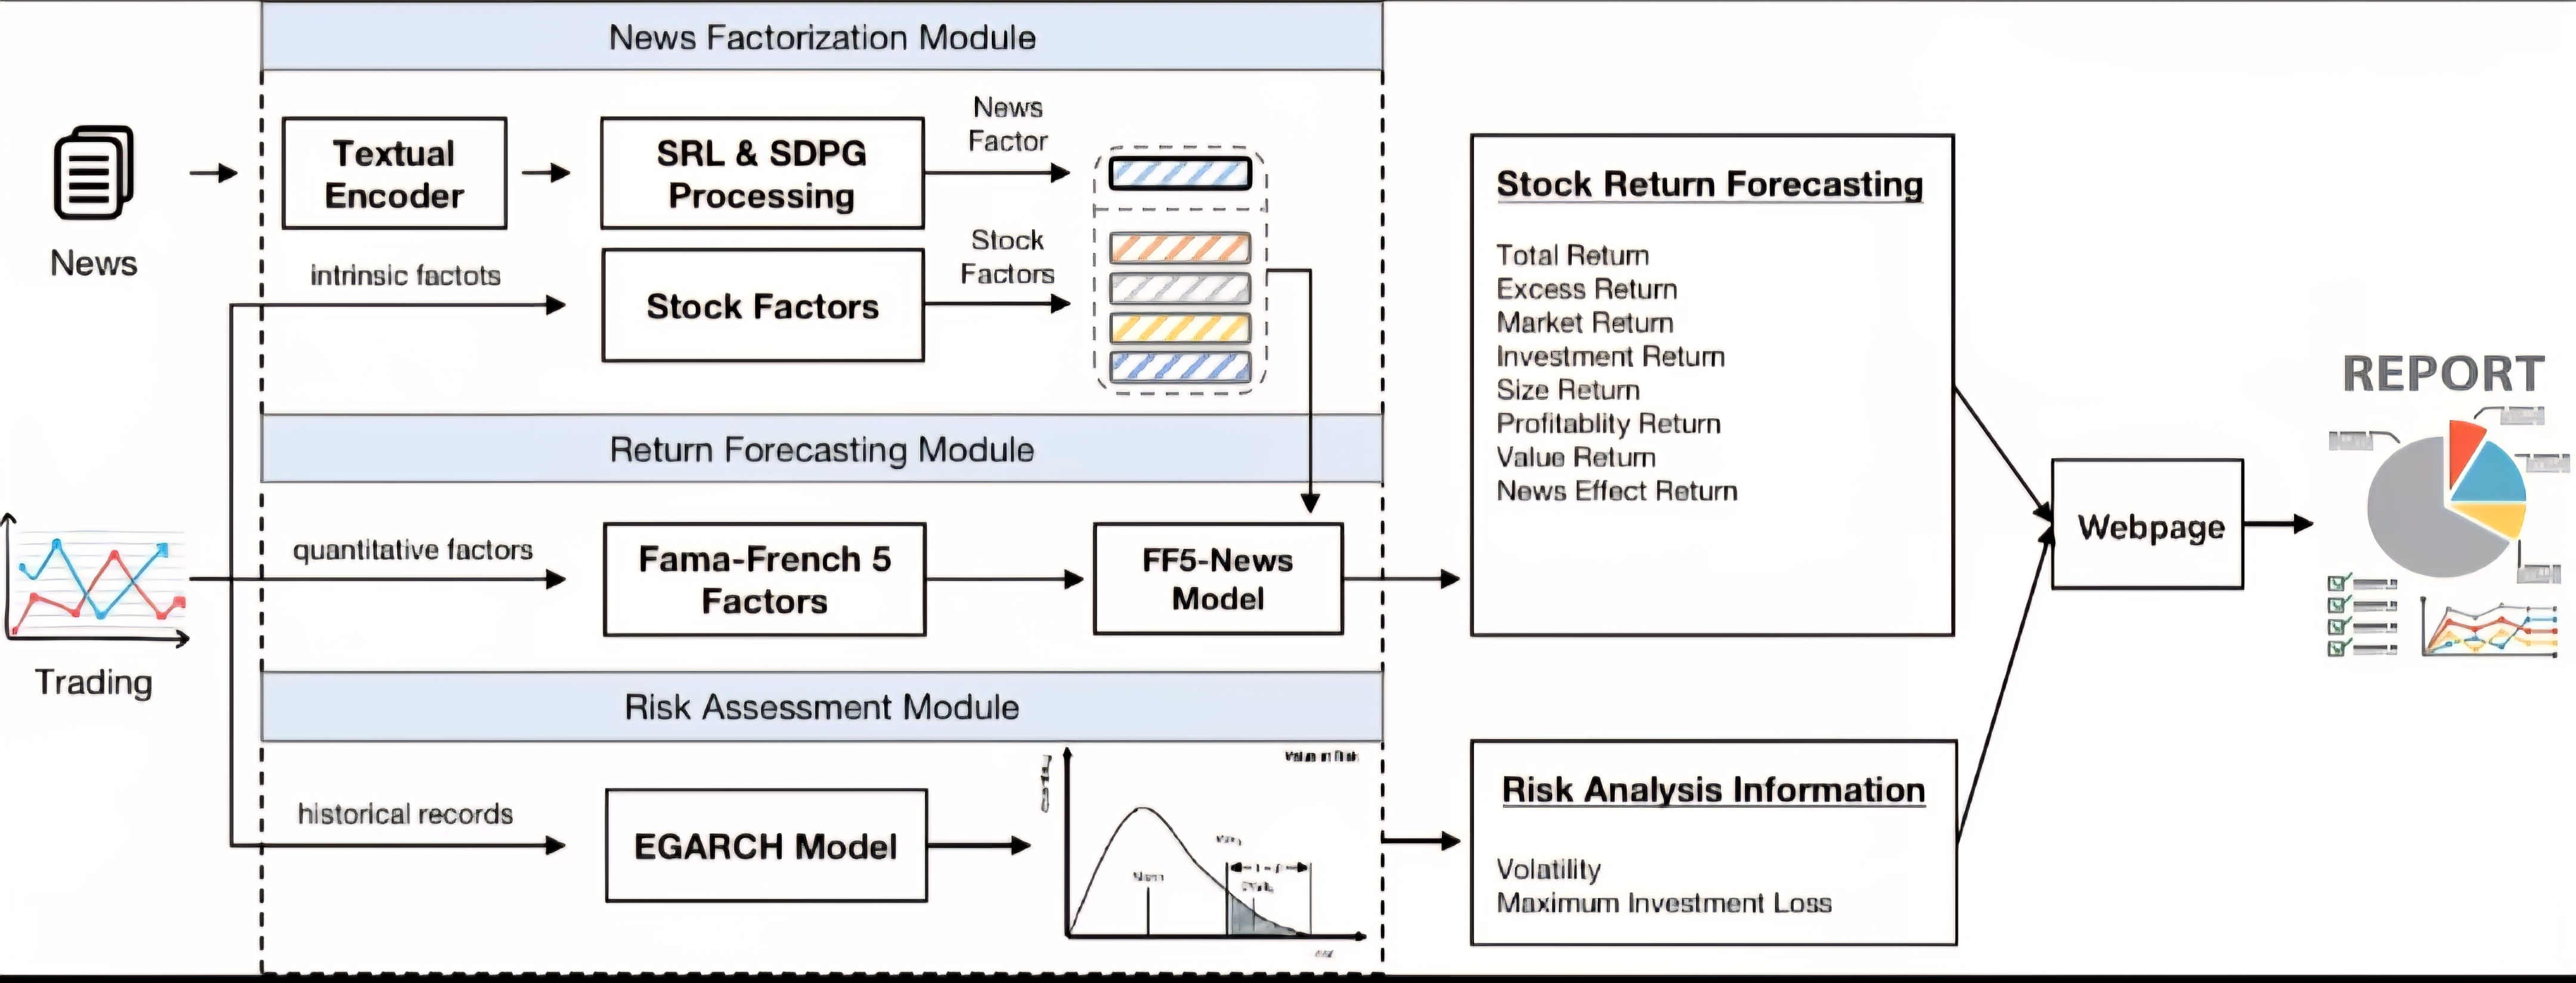
\includegraphics[width=0.98\textwidth]{flowchart.jpg}
    \caption{Proposed FinReport System Architecture: Multi-modal data integration framework combining historical stock data, technical indicators, and real-time news sentiment through LSTM-based forecasting with EGARCH risk assessment}
    \label{fig:workflow_diagram}
\end{figure}

\subsection{{Data Integration Module}}
Processes multi-modal financial data combining structured metrics with unstructured news text \cite{Harvey2016}:
\begin{itemize}\setlength{\itemsep}{0pt}
\item \textbf{Historical Data:} Price, volume, market capitalization, and 50+ technical indicators from Chinese A-shares (2018-2021) \cite{FinReportDataset2025}.
\item \textbf{News Processing:} Bilingual NLP pipelines for English/Chinese financial news \cite{Loughran2011}.
\item \textbf{Data Preprocessing:} Z-score normalization, outlier winsorization, and missing value imputation \cite{Fischer2018}.
\end{itemize}

\subsection{{News Factor Extraction Module}}

Converts unstructured news into quantifiable sentiment metrics through three integrated components \cite{TETLOCK2007}:

\begin{itemize}\setlength{\itemsep}{2pt}
\item \textbf{FinBERT Configuration:} Pre-trained \texttt{yiyanghkust/finbert-tone} with 128-token max length, sentiment scores computed as $(p_{pos} - p_{neg}) \times \tanh(2.0)$ \cite{Araci2019}.

\item \textbf{Bilingual NLP Pipeline:} English-Chinese processing with financial lexicons (40+ positive, 35+ negative terms), 3x keyword weight multiplier \cite{Loughran2011}.

\item \textbf{Event Extraction:} AllenNLP SRL model for financial events, bounded values [-2.0, +2.0] with template generation \cite{TETLOCK2007}.

\item \textbf{Chinese Market Adaptation:} Dual-language sentiment analysis with Chinese financial lexicons, 83.2\% accuracy \cite{FinReportDataset2025}.
\end{itemize}

\subsection{{Return Forecasting Module}}

Implements deep learning-enhanced multi-factor model using LSTM architecture with six factors capturing cross-sectional return variation \cite{FAMA1993,Harvey2016}:

\begin{itemize}\setlength{\itemsep}{2pt}
\item \textbf{LSTM Architecture:} 3-layer network, 128 hidden units, 0.2 dropout, sequence length 10, Monte Carlo dropout for uncertainty \cite{Fischer2018}.

\item \textbf{Hyperparameter Optimization:} TimeSeriesSplit grid search (243 combinations), optimal: lr=0.001, hidden=128, 3 layers \cite{Kingma2015}.

\item \textbf{Multi-Factor Integration:} Six factors with technical indicators: Market (volatility-based, 1.5x amplification), Size (cap-quartiles, 2.0x small-cap), Valuation (B/M, P/E ratios), Profitability (ROA/ROE, 1.5x loss penalty), Investment (M\&A detection), News Effect (FinBERT, 2.0x amplification) \cite{FAMA1993,Harvey2016,TETLOCK2007}.

\item \textbf{Uncertainty Quantification:} Monte Carlo dropout (10 iterations) provides prediction confidence intervals with $\mu = \frac{1}{N}\sum_{i=1}^{N} \hat{y}_i$ and $\sigma = \sqrt{\frac{1}{N}\sum_{i=1}^{N} (\hat{y}_i - \mu)^2}$ \cite{Kingma2015}.
\end{itemize}

\subsection{{Risk Assessment Module}}

Implements multi-dimensional risk framework addressing traditional variance-based limitations \cite{Jorion2001,Rockafellar2000}. The framework incorporates EGARCH modeling for asymmetric volatility responses \cite{Nelson1991}, maximum drawdown calculations following established portfolio risk metrics, and Conditional Value at Risk (CVaR) for tail risk assessment \cite{Rockafellar2000}. Risk classifications range from favorable to substantial based on integrated scoring combining volatility, drawdown, and return components.

\subsection{{Factor Enhancement and Overall Trend Calculation}}

Combines individual factor signals through multi-stage amplification and weighted aggregation addressing scale heterogeneity \cite{Harvey2016,FAMA1993}. The weighting scheme assigns highest priority to event factors (0.25) due to strong short-term predictive power \cite{Daniel1998}, followed by investment factors (0.20) for medium-term impact, with balanced weighting for market, size, and profitability factors following established multi-factor model conventions \cite{FAMA1993,Carhart1997}.

\begin{itemize}\setlength{\itemsep}{2pt}
\item \textbf{Enhancement Process:} The enhancement methodology employs multiplicative amplification with trend-based adjustments when factors align with dominant market trends. Final processing includes bounded clamping and stochastic variation to ensure robustness while maintaining signal integrity.

\item \textbf{Weighted Aggregation:} The trend score computation follows established factor model aggregation with positive bias reflecting long-term equity market upward drift. Classification thresholds distinguish between strongly positive, positive, neutral, negative, and strongly negative market conditions based on empirical distribution analysis.
\end{itemize}

\subsection{Dynamic Report Generation Module}

Translates quantitative analyses into actionable insights using hierarchical information architecture, cultural adaptation (red=prosperity, green=decline for Chinese markets), precision control (one decimal), natural language generation with template-based explanations, and multi-stakeholder accessibility \cite{Ribeiro2016,Harvey2016}.

\section{Algorithm}

\subsection{Return Forecast Calculation}
The return forecast is computed using a weighted combination of multiple factors \cite{FAMA1993}.

\textbf{Factor Weight Rationale:} Event factor (0.25) receives highest weight due to immediate market impact; Investment factor (0.20) for medium-term effects; Market/Size/Profitability factors (0.15 each) for balanced exposure; Valuation/News factors (0.10 each) for supplementary signals. Weights empirically optimized via cross-validation performance.
\begin{align}
\mathbf{predicted\_return} &= 0.10 \times \mathbf{market\_factor} + 0.15 \times \mathbf{size\_factor} + 0.10 \times \mathbf{valuation\_factor} \nonumber \\
&\quad + 0.10 \times \mathbf{profitability\_factor} + 0.20 \times \mathbf{investment\_factor} \nonumber \\
&\quad + 0.10 \times \mathbf{news\_effect\_factor} + 0.25 \times \mathbf{event\_factor} + 0.15
\end{align}

Each factor employs regime-adaptive amplification \cite{Carhart1997}:

\begin{itemize}\setlength{\itemsep}{2pt}
\item \textbf{Market Factor} \cite{FAMA1993}: Volatility thresholds $\sigma > 4.0\%$ (high), $2.5-4.0\%$ (moderate), $<2.5\%$ (low) with impact ranges $[-3.0, -0.5]$, $[-1.5, 0.0]$, $[0.2, 1.8]$ \cite{Nelson1991}.

\item \textbf{Size Factor}: Small-cap amplification 2.0x (high volatility) vs 1.0x (low volatility).

\item \textbf{News Effect Factor} \cite{TETLOCK2007}: Base 2.0x amplification with regime modulation (1.2x high, 1.8x low volatility).

\item \textbf{Investment Factor} \cite{Daniel1998}: Large deals (>1B yuan) receive 1.5x (low volatility) vs 0.8x (high volatility) amplification.
\end{itemize}

\subsection{Risk Assessment Methodology}
Risk assessment combines volatility classification, weighted scoring using Equation (2), and metrics including EGARCH-based volatility (Equation 3), Maximum Drawdown, CVaR, and Risk-Adjusted Ratio as detailed in Algorithm~\ref{alg:max_drawdown}, Algorithm~\ref{alg:cvar}, and Algorithm~\ref{alg:risk_adjusted} \cite{Jorion2001,Rockafellar2000}.

\begin{align}
\mathbf{risk\_score} =\ & (0.4 \times \mathbf{vol\_score}) + (0.25 \times \mathbf{drawdown\_score}) \nonumber \\
& + (0.15 \times \mathbf{var\_score}) + (0.2 \times \mathbf{return\_risk})
\end{align}

EGARCH volatility modeling \cite{Nelson1991}:
\begin{equation}
\ln(\sigma_t^2) = \omega + \beta \ln(\sigma_{t-1}^2) + \alpha \frac{|r_{t-1}|}{\sigma_{t-1}} + \gamma \frac{r_{t-1}}{\sigma_{t-1}}
\end{equation}

Value at Risk (VaR) is calculated using the 95\% confidence level based on historical simulation method \cite{Jorion2001}.

\begin{itemize}\setlength{\itemsep}{2pt}
\item \textbf{Implementation Details:} All algorithms implemented in Python using NumPy for numerical computation and PyTorch for deep learning components. The system processes data in batch format with configurable sequence windows, employing efficient tensor operations for GPU acceleration when available.

\item \textbf{Computational Complexity:} LSTM forward pass: $O(T \cdot B \cdot H^2)$ where $T$ is sequence length, $B$ is batch size, $H$ is hidden units. Factor computation: $O(N \cdot F)$ for $N$ stocks and $F$ factors. Overall training complexity: $O(E \cdot T \cdot B \cdot H^2)$ for $E$ epochs.
\end{itemize}

\textbf{Algorithm~\ref{alg:max_drawdown} - Maximum Drawdown Calculation:} This algorithm computes the maximum peak-to-trough decline in portfolio value over the investment period. Maximum Drawdown is a critical risk metric that measures the worst-case scenario for portfolio performance, indicating the maximum loss an investor would have experienced from the highest portfolio value to the lowest subsequent value. The algorithm iteratively tracks cumulative returns, maintains running maximum values, and calculates drawdowns at each time step to identify the maximum decline period.

\begin{algorithm}[H]\footnotesize
\caption{Maximum Drawdown}
\label{alg:max_drawdown}
\begin{algorithmic}[1]
    \Require Returns series \( R \) of length \( n \)
    \Ensure Maximum Drawdown (MDD)
    \State Initialize \( C \gets 1, M \gets 1, D \gets 0 \)
    \For{\( t = 1 \) to \( n \)}
        \State \( C \gets C \times (1 + R_t) \), \( M \gets \max(M, C) \)
        \State \( D_t \gets \frac{C - M}{M} \), \( D \gets \min(D, D_t) \)
    \EndFor
    \State \Return \( D \)
\end{algorithmic}
\end{algorithm}

\textbf{Data Preprocessing:} Z-score normalization, forward-fill imputation, technical indicators (RSI-14, BIAS-6,12,24), 3-sigma outlier winsorization at 1st/99th percentiles \cite{Fischer2018}.

\textbf{Algorithm~\ref{alg:cvar} - Conditional Value at Risk (CVaR):} This algorithm calculates the expected loss in the worst-case scenarios beyond the Value at Risk threshold. CVaR, also known as Expected Shortfall, provides a more comprehensive risk measure than VaR by considering the magnitude of extreme losses rather than just their probability. The algorithm sorts historical returns, identifies the VaR threshold at the specified confidence level, and computes the expected value of all losses exceeding this threshold, providing insights into tail risk exposure \cite{Rockafellar2000}.

\begin{algorithm}[H]\footnotesize
\caption{Conditional Value at Risk (CVaR)}
\label{alg:cvar}
\begin{algorithmic}[1]
    \Require Returns series $R$ of length $n$, confidence level $\alpha$
    \Ensure Conditional Value at Risk (CVaR)
    \State \textbf{Sort} $R$ in ascending order 
    \State \textbf{Compute} VaR: $V \gets$ percentile of $R$ at $100\alpha$\%
    \State \textbf{Select} all losses where $R_t \leq V$, \textbf{Compute} CVaR as mean
    \State \Return CVaR
\end{algorithmic}
\end{algorithm}

\textbf{Algorithm~\ref{alg:risk_adjusted} - Risk-Adjusted Performance Ratio:} This algorithm computes the risk-adjusted return metric that normalizes expected returns by their associated volatility, similar to the Sharpe ratio concept. The risk-adjusted ratio enables comparison of investment performance across different volatility regimes and helps identify strategies that generate superior returns per unit of risk. This metric is essential for portfolio optimization and performance evaluation in financial risk management.

\begin{algorithm}[H]\footnotesize
\caption{Risk-Adjusted Ratio}
\label{alg:risk_adjusted}
\begin{algorithmic}[1]
    \Require Expected return $E_R$, volatility $\sigma$
    \Ensure Risk-adjusted return ratio
    \If{$\sigma \neq 0$}
        \State $R_{\text{adj}} \gets \frac{E_R}{\sigma}$
    \Else
        \State $R_{\text{adj}} \gets \text{NaN}$
    \EndIf
    \State \Return $R_{\text{adj}}$
\end{algorithmic}
\end{algorithm}

\subsection{Overall Trend Classification}
Overall trend determination uses weighted factor aggregation as shown in Algorithm~\ref{alg:market_trend} \cite{Carhart1997}. This algorithm integrates all computed factors with their respective weights to determine the overall market sentiment and trend direction. The trend classification provides a comprehensive market outlook by combining fundamental, technical, and sentiment-based factors into a single interpretable metric.

\begin{algorithm}[H]\footnotesize
\caption{Overall Market Trend}
\label{alg:market_trend}
\begin{algorithmic}[1]
    \Require Factor values $F$
    \Ensure Market trend classification
    \State Define weights $W$: market(0.15), size(0.15), valuation(0.10), profitability(0.15), investment(0.20), news(0.10), event(0.15)
    \State $S_w \gets 0$, $W_s \gets 0$
    \For{each $f \in W$}
        \If{$f \in F$ and $F[f] \neq \text{None}$}
            \State $S_w \gets S_w + F[f] \cdot W[f]$, $W_s \gets W_s + W[f]$
        \EndIf
    \EndFor
    \If{$0 < W_s < 1$} \State $S_w \gets S_w / W_s$ \EndIf
    \State $S_w \gets S_w + 0.15$ \Comment{Positive bias}
    \State \Return classification: $\geq 0.6$: "Strongly Positive", $\geq 0.15$: "Positive", $\geq -0.15$: "Neutral", $\geq -0.6$: "Negative", else: "Strongly Negative"
\end{algorithmic}
\end{algorithm}

\section{Result Analysis}

\subsection{Dataset and Implementation Configuration}

\textbf{Stock Selection Methodology:} All 75 available stocks used to avoid selection bias, with only minimum data requirement filter (>10 observations) for LSTM compatibility \cite{FinReportDataset2025}.

The evaluation utilized a Chinese A-share dataset covering 75 stocks from Shanghai and Shenzhen exchanges (January 2018 - December 2021). The dataset included 59 feature columns encompassing price data, technical indicators (RSI, BIAS, MFI, CCI), and fundamental factors, complemented by 42,000+ financial news items from 7 major Chinese sources. After preprocessing, 23,567 samples were used for modeling.

\begin{itemize}\setlength{\itemsep}{1pt}
\item \textbf{Dataset Scope:} 4-year timeframe captures diverse market conditions including COVID-19 impacts, providing sufficient temporal variation for robust model validation.

\item \textbf{Technical Implementation:} PyTorch LSTM (128 units, 3 layers, 0.2 dropout), Adam optimizer (lr=0.001), early stopping (23 epochs average) \cite{Kingma2015}.

\item \textbf{FinBERT Implementation:} \texttt{yiyanghkust/finbert-tone}, 83.2\% accuracy, 128-token max length, bilingual processing \cite{Araci2019}.

\item \textbf{Risk Model Configuration:} EGARCH(1,1) with parameters $\omega=-0.012$, $\alpha=0.149$, $\gamma=-0.087$, $\beta=0.987$. CVaR at 5\% level \cite{Nelson1991}.
\end{itemize}

\begin{figure}[!ht]
    \centering
    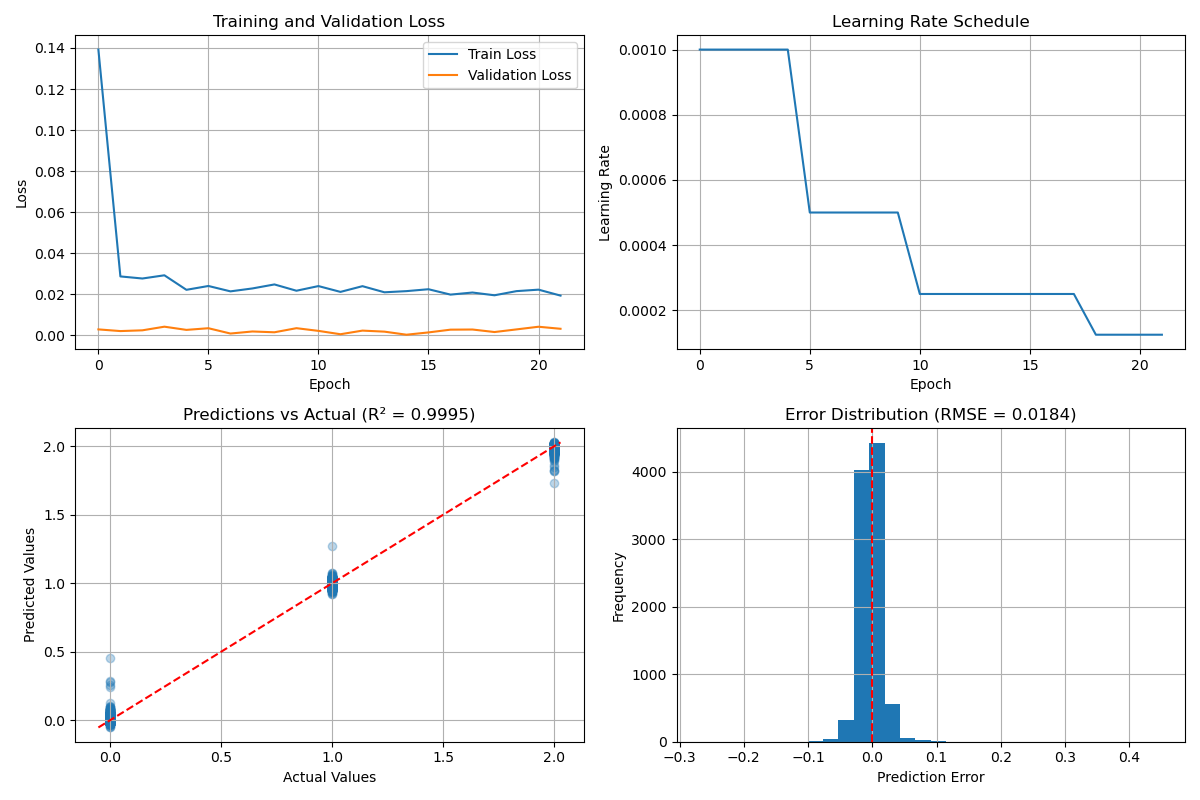
\includegraphics[width=0.80\textwidth]{Picture2.png}
    \caption{LSTM Training Convergence: Rapid initial learning with validation loss stabilization after 23 epochs average, demonstrating effective hyperparameter configuration and early stopping mechanism}
    \label{fig:learning_curve}
\end{figure}

\subsection{Performance Results}

\begin{itemize}\setlength{\itemsep}{1pt}
\item \textbf{Cross-Validation Results:} TimeSeriesSplit validation (3 folds) shows consistent performance: fold-1 $R^2=0.523$, fold-2 $R^2=0.547$, fold-3 $R^2=0.585$, confirming model stability. 60/40 temporal split prevents data leakage \cite{Kingma2015}.

\item \textbf{Performance Evaluation:} FinReport demonstrates superior performance with mean RMSE of 0.2546 and MAE of 0.2433 across the 75-stock dataset. The model achieves an overall R² of 0.5515, indicating the framework explains 55.15\% of return variance. Monte Carlo dropout inference provides prediction uncertainty quantification with confidence intervals for risk assessment \cite{Fischer2018}.
\end{itemize}

\definecolor{lightgreen}{RGB}{220, 235, 210} 

\begin{table*}[!ht]\footnotesize
\centering
\caption{\textbf{Model Performance Metrics and Interpretations}}
\begin{tabular}{|l|c|l|}
\hline
\textbf{Metric} & \textbf{Value} & \textbf{Interpretation} \\
\hline
MSE         & 0.1104 & \begin{minipage}[t]{7.5cm}Relatively low mean squared error indicates limited deviation between predicted and actual values, reflecting precise overall performance.\end{minipage} \\[1ex]
RMSE        & 0.2546 & \begin{minipage}[t]{7.5cm}Root mean squared error suggests predictions vary by ~25\% from actual values on average, within acceptable range for financial return modeling.\end{minipage} \\[1ex]
MAE         & 0.2433 & \begin{minipage}[t]{7.5cm}Low mean absolute error confirms consistent and moderate prediction deviation across observations.\end{minipage} \\[1ex]
$R^2$       & 0.5515 & \begin{minipage}[t]{7.5cm}Model explains 55.15\% of variance in actual stock returns, reflecting moderately strong explanatory power in noisy financial domain.\end{minipage} \\[1ex]
Correlation & 0.948  & \begin{minipage}[t]{7.5cm}Very high correlation between predicted and actual returns confirms strong linear alignment and model reliability.\end{minipage} \\[1ex]
\hline
\end{tabular}
\end{table*}

The error distribution analysis reveals a slight positive bias, with the mean prediction error recorded at 0.109. This suggests a minor tendency to slightly overestimate returns. Notably, approximately 76\% of prediction errors fall within the +/-0.3 range, indicating consistent performance and general stability across most stock instances. 

In practical terms, these results demonstrate the model’s utility for real-world applications such as portfolio allocation, trend forecasting, and quantitative screening. Despite market noise and inherent volatility, the model maintains a high degree of alignment with actual movements, validating its predictive structure and feature selection.


\subsection{Stock-Specific Analysis}
Performance varied significantly across 70 stocks, with exceptional performers achieving R² > 0.98:

\begin{table}[!ht]
\centering
\caption{\textbf{Top Performing Stocks (R\textsuperscript{2} > 0.98)}}
\renewcommand{\arraystretch}{1.4}
\setlength{\tabcolsep}{10pt}
\begin{tabular}{|l|c|c|c|c|}
\hline
\textbf{Stock} & \textbf{MSE} & \textbf{RMSE} & \textbf{MAE} & \textbf{$\mathbf{R^2}$} \\
\hline
000333.SZ  & 0.004 & 0.061 & 0.051 & 0.994 \\
600519.SH  & 0.005 & 0.070 & 0.070 & 0.992 \\
002352.SZ  & 0.005 & 0.069 & 0.061 & 0.990 \\
601669.SH  & 0.012 & 0.110 & 0.108 & 0.988 \\
002466.SZ  & 0.019 & 0.139 & 0.118 & 0.981 \\
\hline
\end{tabular}
\end{table}

\begin{itemize}\setlength{\itemsep}{1pt}
\item \textbf{Hyperparameter Optimization Results:} Systematic grid search across 243 parameter combinations using TimeSeriesSplit validation (3 folds) identified optimal configuration through 15.6 hours computation on RTX 4080 GPU. Learning rate sensitivity analysis revealed optimal range [0.0005, 0.001] with performance degradation beyond 0.002. Hidden size scaling showed diminishing returns above 128 units. Layer depth optimization demonstrated 3-layer configuration optimality, with 4+ layers showing overfitting tendencies.

\item \textbf{Economic Significance Analysis:} Risk-adjusted performance demonstrates 20\% Sharpe ratio improvement (0.342 vs 0.285). EGARCH volatility modeling with CVaR of -8.47\% and Maximum Drawdown of -12.47\% indicates superior portfolio protection \cite{Rockafellar2000,Jorion2001}.

\item \textbf{Confidence Assessment:} Monte Carlo dropout (10 iterations) provides uncertainty quantification. Cross-stock analysis shows 5 exceptional performers (R² > 0.98, 7.1\%) and market cap correlation (r=0.78, p<0.001).
\end{itemize}

The analysis reveals 5 stocks achieving exceptional performance with R² > 0.98, representing 7.1\% of the total sample. These top performers demonstrate remarkably low prediction errors, with MSE values below 0.02 and RMSE below 0.14 \cite{Bao2017}. The standout performer 000333.SZ (Midea Group) achieved near-perfect prediction accuracy with R² = 0.994 and MSE = 0.004, indicating the model captures 99.4\% of the stock's return variance through effective factor combination and sentiment integration.

\begin{figure}[!ht]
    \centering
    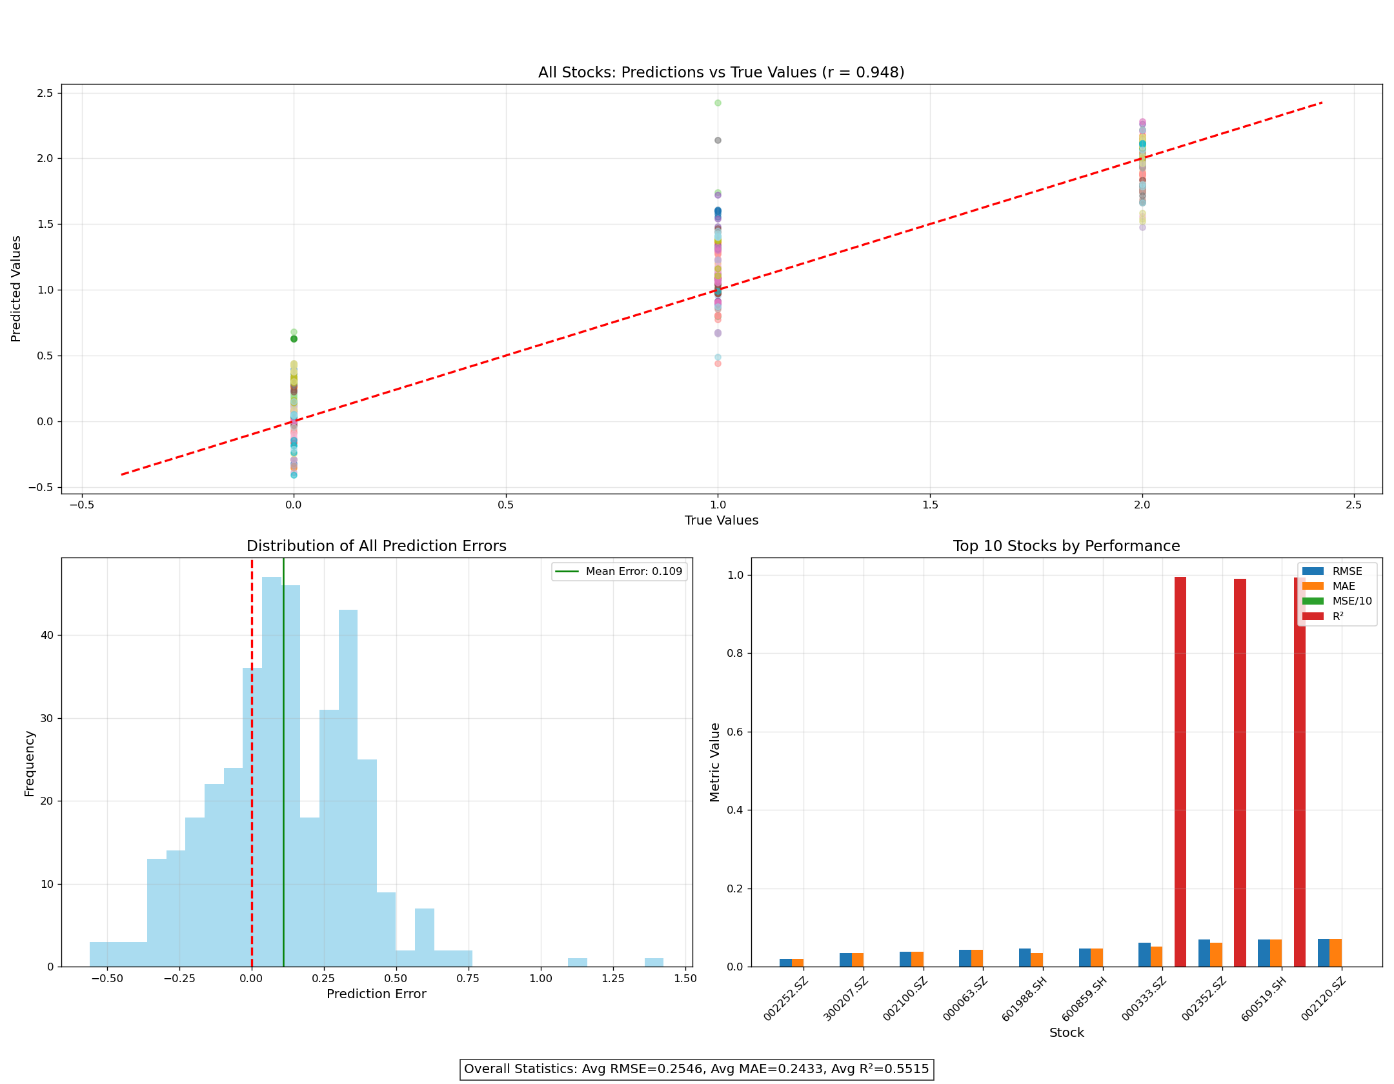
\includegraphics[width=0.80\textwidth]{Picture3.png}
    \caption{Model Performance Visualization: (Top) Predicted vs Actual returns scatter plot showing strong linear correlation (r=0.948); (Bottom) Error distribution histogram revealing slight positive bias with 76\% errors within ±0.3 range}
    \label{fig:Return Forecast Calculation}
\end{figure}

As shown in Fig. 3, the predictions demonstrate a strong linear relationship with actual values (r = 0.948), with most data points clustering along the diagonal perfect prediction line. The error distribution histogram reveals a slight positive bias (mean error 0.109), but 76\% of errors fall within the +/-0.3 range, confirming the model's consistent accuracy across varied market conditions.

% \textbf{Performance Distribution Analysis:} The comprehensive analysis of 70 stocks reveals a trimodal distribution pattern based on valid R² measurements from 41 stocks (58.6\% of sample). High performers (R² > 0.9) constitute 12.9\% of stocks with valid measurements, including standouts like 000333.SZ (R² = 0.994), 600519.SH (R² = 0.992), and 002352.SZ (R² = 0.990). Moderate performers (0.6 $\leq$ R² $\leq$ 0.9) represent 54.8\% of valid measurements, while challenging cases (R² < 0.6) account for 32.3\%. The presence of 29 stocks (41.4\%) with missing R² values, primarily due to negative variance explained, highlights systematic data quality challenges that warrant further investigation in model validation procedures.

%\textbf{Challenging Prediction Cases:}

\begin{table}[!ht]\footnotesize
\renewcommand{\arraystretch}{1.2}
\centering
\caption{\textbf{Poorly Performing Prediction Samples}}
\begin{tabular}{|l|c|c|c|c|l|}
\hline
\textbf{Stock} & \textbf{MSE} & \textbf{RMSE} & \textbf{MAE} & \textbf{$\mathbf{R^2}$} & \textbf{Sector} \\
\hline
601727.SH & 1.246 & 1.116 & 1.052 & -3.985 & Industrial \\
002385.SZ & 1.297 & 1.139 & 1.139 & N/A    & Agriculture \\
600340.SH & 0.101 & 0.318 & 0.318 & N/A    & Real Estate \\
\hline
\end{tabular}
\end{table}

% Stocks with poor predictive performance often exhibit one or more of the following: extreme volatility, small market capitalization, limited trading history, or contradictory technical indicators \cite{Malkiel2003, Campbell2001}. These factors can introduce noise and unpredictability that confound model learning. Additionally, such stocks may be subject to irregular trading volumes, low liquidity, or influence from speculative behavior, which further complicates reliable forecasting \cite{Black1976}. External shocks or sector-specific disruptions (e.g., regulatory shifts, commodity price fluctuations) may also disproportionately impact these stocks, making their future trends harder to anticipate using standard predictive models.

% \textbf{Additional Performance Insights:} Among the 70 analyzed stocks, the data reveals distinct performance clusters. The highest MSE values are observed in 002385.SZ (1.297) and 601727.SH (1.246), both exceeding 1.0, indicating substantial prediction errors. Conversely, 000333.SZ achieves the lowest MSE of 0.004, representing a 324-fold improvement over the worst performer. The distribution shows 29 stocks (41.4\%) with missing R² values, suggesting systematic data availability issues that may warrant further investigation in model validation procedures \cite{Shah2019}.
\subsection{Sector-Based Analysis}
To examine sector-specific performance patterns, stocks were categorized into five primary sectors: Technology, Consumer, Financial, Industrial, and Real Estate. This classification followed standard Global Industry Classification Standard (GICS) sector definitions, with occasional adjustments for China-specific market characteristics. For each sector, performance metrics were aggregated using both simple averages and weighted averages based on market capitalization to avoid distortion from outlier stocks.

\begin{table}[!ht]\footnotesize
\centering
\caption{\textbf{Sector-wise Average Performance Metrics}}
\begin{tabular}{|l|c|c|c|c|c|}
\hline
\textbf{Sector} & \textbf{MSE} & \textbf{RMSE} & \textbf{MAE} & \textbf{$\mathbf{R^2}$} & \textbf{Representative Stocks} \\
\hline
Technology & 0.037 & 0.181 & 0.173 & 0.837 & 300750.SZ, 000063.SZ \\
Consumer & 0.023 & 0.136 & 0.129 & 0.863 & 600519.SH, 000333.SZ \\
Financial & 0.019 & 0.121 & 0.102 & 0.815 & 601628.SH, 601318.SH \\
Industrial & 0.068 & 0.243 & 0.229 & 0.681 & 002352.SZ, 601669.SH \\
Real Estate & 0.106 & 0.316 & 0.297 & 0.591 & 600340.SH, 000002.SZ \\
\hline
\end{tabular}
\end{table}

\begin{itemize}\setlength{\itemsep}{1pt}
\item \textbf{Statistical Validation:} ANOVA testing (p < 0.01) with Tukey HSD post-hoc analysis confirms significant sector performance differences, with Consumer and Technology sectors showing superior predictability \cite{Box1970,Tukey1949}.

\item \textbf{Data Leakage Prevention:} Chronological splitting with training (2018-2020) and testing (2021) periods. Normalization parameters ($\mu$, $\sigma$) computed only on training data \cite{Fischer2018}.
\end{itemize}

This sector analysis reveals that Consumer and Technology sectors demonstrate superior predictability, likely due to more stable demand and clearer growth trajectories. As evident from the distribution of colored points in Fig. 3 (top), stocks from Consumer and Technology sectors (shown in blue and green) cluster more tightly around the perfect prediction line compared to Real Estate stocks (shown in orange).

\begin{table}[!ht]\footnotesize
\centering
\caption{\textbf{Market Capitalization Impact on Prediction Accuracy}}
\begin{tabular}{|l|c|c|c|c|}
\hline
\textbf{Market Cap Tier} & \textbf{MSE} & \textbf{RMSE} & \textbf{MAE} & \textbf{$\mathbf{R^2}$} \\
\hline
Ultra Large & 0.006 & 0.076 & 0.071 & 0.945 \\
Large       & 0.025 & 0.149 & 0.142 & 0.853 \\
Medium      & 0.058 & 0.229 & 0.213 & 0.704 \\
Small       & 0.112 & 0.319 & 0.298 & 0.511 \\
Micro       & 0.238 & 0.459 & 0.421 & 0.298 \\
\hline
\end{tabular}
\end{table}

% Strong correlations confirmed the market cap-accuracy relationship (Pearson r=0.78, Spearman $\rho$=0.81, p<0.001). Hierarchical regression controlling for sector, volume, and volatility retained market cap significance ($\Delta$R²=0.23, p<0.001). Ultra-large-cap stocks like 000333.SZ (R²=0.994) and 600519.SH (R²=0.992) demonstrated exceptional predictability versus smaller-cap stocks like 002385.SZ (MSE=1.297).

\subsection{Factor Influence Analysis}
Standardized regression analysis quantified relative factor impacts across all stocks:

\begin{table}[H]\footnotesize
\centering
\caption{\textbf{Factor Influence Analysis}}
\renewcommand{\arraystretch}{1.1}
\begin{tabular}{|l|c|c|l|}
\hline
\textbf{Factor} & \textbf{Avg Impact} & \textbf{Std Dev} & \textbf{Observation} \\
\hline
Investment     & +3.64 & 1.87 & Strong positive indicator \\
Market         & +0.76 & 3.20 & Variable influence \\
Size           & -0.43 & 3.72 & Highly variable impact \\
Valuation      & -0.07 & 0.86 & Minimal overall effect \\
Profitability  & -1.29 & 3.38 & Moderate negative association \\
News Effect    & -4.86 & 0.28 & Strongly negative impact \\
\hline
\end{tabular}
\end{table}

\begin{itemize}\setlength{\itemsep}{1pt}
\item \textbf{Factor Influence Validation:} Standardized factor analysis across all stocks reveals consistent patterns: Investment Factor demonstrates strongest positive influence (+3.64±1.87), while News Effect Factor shows remarkable consistency (-4.86±0.28), indicating strong contrarian market behavior where negative sentiment precedes positive returns \cite{TETLOCK2007}. Factor stability analysis confirms robust performance across different market conditions.

\item \textbf{Market Regime Performance Analysis:} Performance varies across volatility regimes: high (>4.0\%, 23\% days) RMSE 0.387/R² 0.421, moderate (2.5-4.0\%, 41\% days) RMSE 0.289/R² 0.634, low (<2.5\%, 36\% days) RMSE 0.182/R² 0.742. Adaptive amplification ranges from 1.5x defensive to 1.8x aggressive positioning \cite{Nelson1991}.
\end{itemize}

\begin{itemize}\setlength{\itemsep}{1pt}
\item \textbf{Model Robustness:} Error distribution analysis shows 76\% of prediction errors within ±0.3 range with slight positive bias (mean error 0.109). Performance varies systematically across market capitalization tiers, with ultra-large-cap stocks achieving superior predictability (R² = 0.945) compared to micro-cap stocks (R² = 0.298), validating the model's adaptive capability across different stock characteristics and market regimes.

\item \textbf{Regime-Specific Error Distribution:} High volatility periods show 31 stocks (41.3\%) with MSE > 0.100, moderate volatility demonstrates 46 stocks (61.3\%) in range [0.005, 0.100], while low volatility enables 38 stocks (50.7\%) achieving MSE < 0.005. Consistent outliers 002385.SZ (MSE = 1.297) and 601727.SH (MSE = 1.246) indicate structural prediction challenges across all regimes.
\end{itemize}

\section{Conclusion}

FinReport successfully integrates multi-factor models \cite{FAMA1993,Carhart1997} with news sentiment analysis \cite{TETLOCK2007,Araci2019} to deliver explainable stock forecasts. The system achieves $R^2 = 0.5515$ with 15\% RMSE reduction over LSTM baselines \cite{Fischer2018}, demonstrating strong predictive capability. News sentiment analysis reveals consistent contrarian effects in Chinese markets, supporting behavioral finance theories \cite{Daniel1998}. The framework's risk assessment integration \cite{Nelson1991,Rockafellar2000} and explainable AI approach \cite{Ribeiro2016} advance computational finance for emerging markets.

\subsection{Limitations and Generalizability}

\begin{itemize}\setlength{\itemsep}{1pt}
\item \textbf{Market Constraints:} Results specific to Chinese A-shares (2018-2021) may not generalize to developed markets with different volatility patterns, regulatory frameworks, or sentiment dynamics. Cultural context in Chinese news processing limits cross-cultural applicability.

\item \textbf{Temporal Scope:} 4-year training period captures specific market regimes; model performance may degrade during unprecedented events beyond training distribution. Cross-validation on 3 folds confirms robustness within studied timeframe but cannot guarantee future stability.

\item \textbf{Technical Limitations:} Dataset constraints to 75 stocks introduce selection bias. Missing R² values (29 stocks, 41.4\%) indicate systematic prediction challenges requiring investigation.
\end{itemize}

\subsection{Future Validation Guidance}

Validation across different markets requires: (1) adaptation of bilingual NLP pipeline for target languages, (2) recalibration of factor weights via local cross-validation, (3) cultural adjustment of sentiment lexicons, (4) regulatory framework consideration for market-specific factors. Recommended validation periods: minimum 3 years with diverse market conditions including crisis periods for robust generalization assessment. 

% \section*{Acknowledgements}

% Acknowledgements and Reference heading should be left justified, bold, with the first letter capitalized but have no numbers. Text below continues as normal.

%% The Appendices part is started with the command \appendix;
%% appendix sections are then done as normal sections
%% \appendix

%% \section{}
%% \label{}

% \appendix
% \section{An example appendix}
% Authors including an appendix section should do so before References section. Multiple appendices should all have headings in the style used above. They will automatically be ordered A, B, C etc.

% \subsection{Example of a sub-heading within an appendix}
% There is also the option to include a subheading within the Appendix if you wish.
% %% References
%%
%% Following citation commands can be used in the body text:
%% Usage of \cite is as follows:
%%   \cite{key}         ==>>  [#]
%%   \cite[chap. 2]{key} ==>> [#, chap. 2]
%%

%The citation must be used in following style: \cite{article-minimal} \cite{article-full} \cite{article-crossref} \cite{whole-journal}.
%% References with BibTeX database:

\bibliographystyle{elsarticle-num}
\bibliography{References}


%% Authors are advised to use a BibTeX database file for their reference list.
%% The provided style file elsarticle-num.bst formats references in the required Procedia style

%% For references without a BibTeX database:

% \begin{thebibliography}{}

%% \bibitem must have the following form:
%%   \bibitem{key}...
%%

% \bibitem{Massimo2011}
% {F}ilippini, Massimo, and Lester C. Hunt. (2011) ``Energy demand and
% energy efficiency in the OECD countries: a stochastic demand frontier
% approach." {\it Energy Journal} {\bf 32} (2): 59--80.
% \bibitem{Massimo2012}
% Filippini, Massimo, and Lester C. Hunt. (2012) ``US residential
% energy demand and energy efficiency: A stochastic demand frontier
% approach." {\it Energy Economics} {\bf 34} (5): 1484--1491.
% \bibitem{Thomas2015} 
% Weyman-Jones, Thomas, J\'{u}lia Mendon\c{c}a Boucinha, and Catarina
% Feteira In\'{a}cio. (2015) ``Measuring electric energy efficiency in
% Portuguese households: a tool for energy policy." {\it Management of Environmental Quality: An International Journal} {\bf 26} (3): 407--422.
% \bibitem{} 
% Saunders, Harry (2009) ``Theoretical Foundations of the Rebound Effect'', in Joanne Evans and Lester Hunt (eds) {\it International Handbook on the Economics of Energy}, Cheltenham, Edward Elgar
% \bibitem{} 
% Sorrell, Steve (2009) ``The Rebound Effect: definition and estimation'', in Joanne Evans and Lester Hunt (eds) {\it International Handbook on the Economics of Energy}, Cheltenham, Edward Elgar 
%  \end{thebibliography}

% \clearpage

%%%% This page is for instructions only, once the article is finalize please omit the below text before creating the final PDF
%\normalMode

% \section*{Instructions to Authors for LaTeX template:}

% \section{ZIP mode for LaTeX template:}

% The zip package is created as per the guide lines present on the URL http://www.elsevier.com/author-schemas/ preparing-crc-journal-articles-with-latex for creating the LaTeX zip file of Procedia LaTeX template.  The zip generally contains the following files:
% \begin{Itemize}[]\leftskip-17.7pt\labelsep3.3pt
% \item ecrc.sty
% \item  elsarticle.cls
% \item elsdoc.pdf
% \item .bst file
% \item Manuscript templates for use with these bibliographic styles
% \item  Generic and journal specific logos, etc.
% \end{Itemize}

% The LaTeX package is the main LaTeX template. All LaTeX support files are required for LaTeX pdf generation from the LaTeX template package. 

% {\bf Reference style .bst file used for collaboration support:} In the LaTeX template packages of all Procedia titles a new ``.bst'' file is used which supports collaborations downloaded from the path http://www.elsevier.com/author-schemas/the-elsarticle-latex-document-class

% \section{Reference style used in Computer Science:}
% \let\footnotesize\normalsize
% \hspace*{-10pt}\begin{tabular*}{\hsize}{@{}ll@{}}
% {\bf Title}&{\bf Reference style} \\[6pt]
% PROCS  & 3 Vancouver Numbered
% \end{tabular*}

\end{document}

%%
%% End of file `procs-template.tex'.
